\newcommand{\h}[1]{\textbf{#1}}
\newcommand{\basePhyLayer}{BasePhyLayer}
\newcommand{\baseMacLayer}{BaseMacLayer}


\section{modelling}

\subsection{overview}

Here we present the design- and interface details of the OMNeT-module \h{\basePhyLayer} and go step-by-step through the requirement specification:

\begin{enumerate}
 \item internal class diagram of \h{\basePhyLayer} and relation (pointers, references and OMNeT-gates) to \h{\baseMacLayer}
 \item interface description for all involved \textsf{C++}-classes
 \item flow charts for reception of MacPacket from upper layer and AirFrame from the channel
 \item detailed flow chart for the receiving process
\end{enumerate}

\subsection{classgraph}

We start with the classgraph for the OMNeT-module \h{\basePhyLayer} that shows its
\textsf{C++}-classes, relations to other OMNeT-modules (especially \h{\baseMacLayer})
and OMNeT-messages sent between them.

The \h{\basePhyLayer} hold a list\req{analogueMulti} of AnalogueModels and a pointer to a Decider. Thus the AnalogueModel and the Decider are submodules of \h{\basePhyLayer}. This way one is able to change\req{analogueExtensible}\req{deciderExtensible} and replace\req{analogueIndependent}\req{deciderIndependent} them independently from the \h{\basePhyLayer}.

\begin{figure}[H]
 \centering
 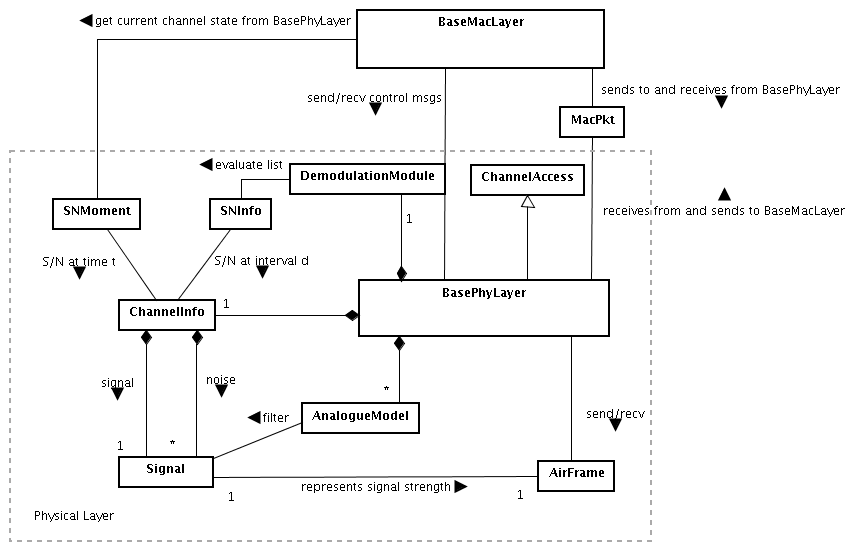
\includegraphics[width=400pt]{modelling/class_diagram.png}
 \caption{class graph}
 \label{fig: classgraph}
\end{figure}
\newpage

\subsection{The \h{\basePhyLayer} interface}

In this section we focus on how one is able to communicate with the \h{\basePhyLayer}, i.e. 
especially the \h{\baseMacLayer}. 
The \h{\baseMacLayer} is connected by a control channel to the \h{\basePhyLayer}. Over this channel the 
\h{\basePhyLayer} can inform the \h{\baseMacLayer} about specific events\req{provactive} (like the transmission over event).

Additionaly \h{\baseMacLayer} holds a reference to the \h{\basePhyLayer}. With this reference \h{\baseMacLayer} can obtain information\req{provpassive} about the channelstate\req{channelstate} and the current mode\req{currentmode}. Further it is able to set current mode in \h{\basePhyLayer} via method call\req{switchmode}.

\begin{figure}[H]
 \centering
 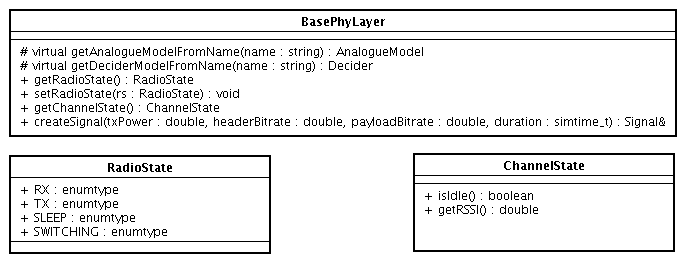
\includegraphics[width=340pt]{modelling/BasePhyLayer_members.png}
 \caption{BasePhyLayer interface}
 \label{fig: BasePhyLayer interface}
\end{figure}
\newpage


\subsection{AnalogueModel and Signal}

The Signal represents the function of signal strength over time of an AirFrame. 
The AnalogueModel is designed as a filter which can be applied at a Signal\req{analogueFilter}.
This way attenuation effects like pathloss\req{analogueSimPathloss}, shadowing\req{analogueSimShadowing} and fading\req{analogueSimFading} can be implemented as a concrete AnalogueModel which changes a given Signal appropriatly.

\begin{figure}[H]
 \centering
 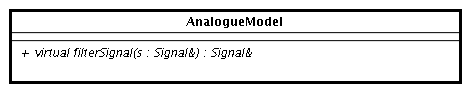
\includegraphics[width=340pt]{modelling/AnalogueModel_members.png}
 \caption{analogue model interface}
 \label{fig: analogue model interface}
\end{figure}

To be able to filter a referenced signal in a specified interval or at a specific point in time, the AnalogueModel gets an iterator from the Signal.

\begin{quote}
\emph{BEWARE: Anyone who subclasses Signal should make shure to have a properly
working SignalTimeIterator (subclassed) for it. The SignalTimeIterator should always
iterate over \textit{every} timestamp in each dimension. This way simple filters can be reused for multidimensional Signals.}
\end{quote}

\begin{figure}[H]
 \centering
 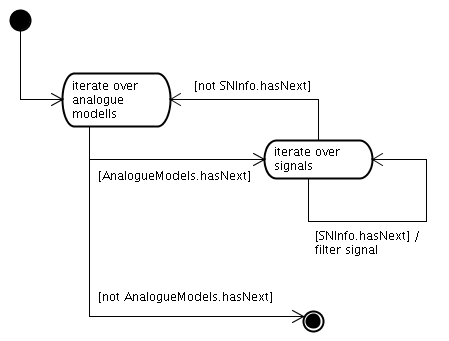
\includegraphics[width=300pt]{modelling/apply_analogue_modells_detail.png}
 \caption{application of analogue models}
 \label{fig: application analogue models}
\end{figure}
\newpage

\subsection{Decider}

The decider provides one method to decide wether a packet could be interpreted as Signal or it is only noise\req{rcvClassify}. And another method to decide if a packet was received correctly\req{rcvIsCorrect}.

The deciders performs both tasks by evaluating the Signals and noise during a certain interval. This Signal and noise information is hold inside the SNInfo class (see  \ref{SNInfoModelling}).

To be able to provide additional information (like bit wise errors\req{deciderBitwise}) besides the information if the packet is correct, the Decider returns a DeciderResult.

\begin{figure}[H]
 \centering
 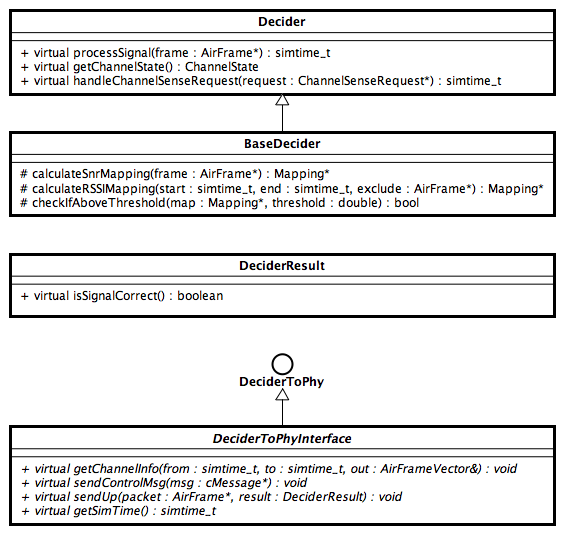
\includegraphics[width=340pt]{modelling/DeciderModule_members.png}
 \caption{Decider interface}
 \label{fig: Decider interface}
\end{figure}
\newpage

\subsection{SNInfo and ChannelInfo}
\label{SNInfoModelling}

ChannelInfo keeps track of all AirFrames on the channel. It does not differ between \textit{signal} and \textit{noise}. \h{\basePhyLayer} is able to
add and remove references to certain AirFrames.

ChannelInfo is able to record the whole channel over time from a start to a stop signal and can return a vector of Signals (references) that intersect with a given time interval.\\
SNInfo is created by \h{\basePhyLayer} when a packet arrives to collect all signals from the channel that intersect with the reception time interval of the packet.

\begin{figure}[H]
 \centering
 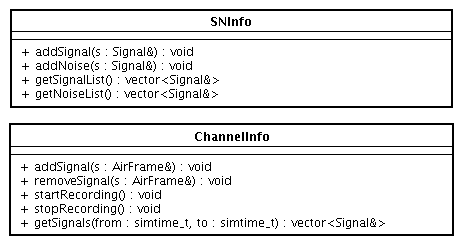
\includegraphics[width=340pt]{modelling/ChannelInfo_members.png}
 \caption{channel details}
 \label{fig: channel details}
\end{figure}

\newpage

\subsection{AirFrame}


\begin{figure}[H]
 \centering
 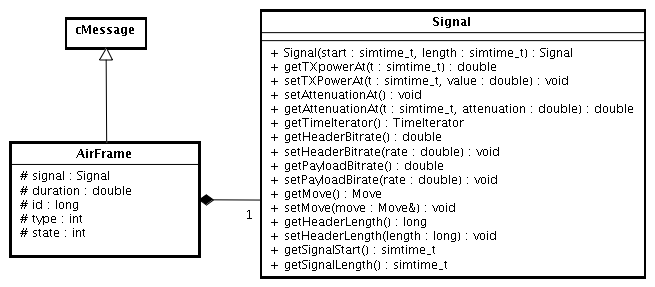
\includegraphics[width=300pt]{modelling/AirFrame_members.png}
 \caption{member arrangement in AirFrame and Signal}
 \label{fig: member AirFrame}
\end{figure}
\newpage

\subsection{receiving a MacPkt}

The class MacToPhyControlInfo is designed as the container for control info\req{packetFromMac} the \h{\baseMacLayer} wants to attach to the packet given down to \h{\basePhyLayer} for sending.

The packet itself is handed down as a MacPkt via OMNeT-channel. 

\begin{figure}[h]
 \centering
 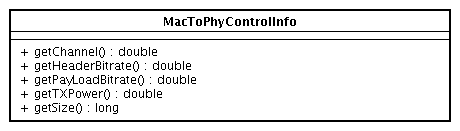
\includegraphics[width=340pt]{modelling/MacToPhyCtrlInfo_members.png}
 \caption{MacToPhyControlInfo interface}
 \label{fig: MacToPhyCtrlInfo interface}
\end{figure}

\begin{figure}[H]
 \centering
 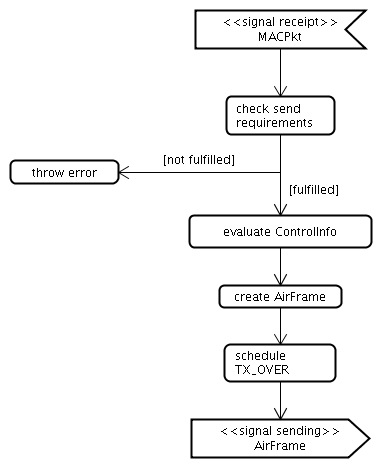
\includegraphics[width=300pt]{modelling/onMACPkt.png}
 \caption{sending process}
 \label{fig: sending process}
\end{figure}

\subsection{Receiving and processing an AirFrame}

The reception of an AirFrame is divided into:
\begin{enumerate}
	
	\item optional propagation delay\req{rcvSimDelay},
	\item reception of the preamble\req{rcvSimPreamble},
	\item application of AnalogueModels to the corresponding SNInfo of the preamble\req{rcvFilterPreamble},
	\item decision whether packet is considered noise (Decider),
	\item reception of the packet\req{rcvSimDuration}.
\end{enumerate}

Afterwards the packet is dropped if it was noise. Otherwise Signal and all interfering noise is collected within a SNInfo, filtered by the analogue models\req{rcvFilterSignals} and then proceeded to the Decider to decide if it was received correctly. If the result turns out positive, the MacPkt inside the AirFrame is decapsulated and send to the \h{\baseMacLayer}\req{rcvPassToMAC}.

\begin{figure}[H]
 \centering
 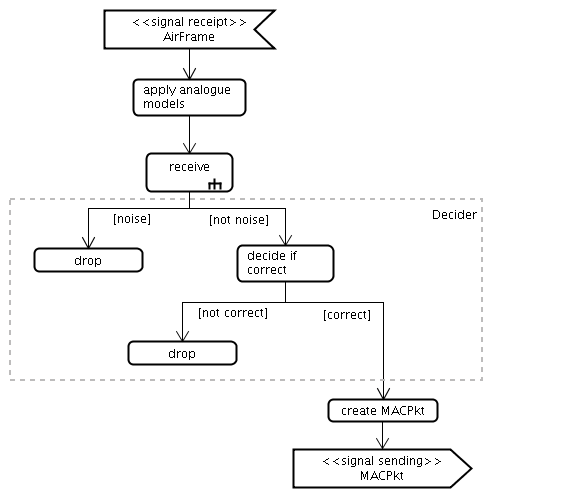
\includegraphics[width=340pt]{modelling/onAirFrame.png}
 \caption{receiving process}
 \label{fig: receiving process}
\end{figure}

\begin{figure}[H]
 \centering
 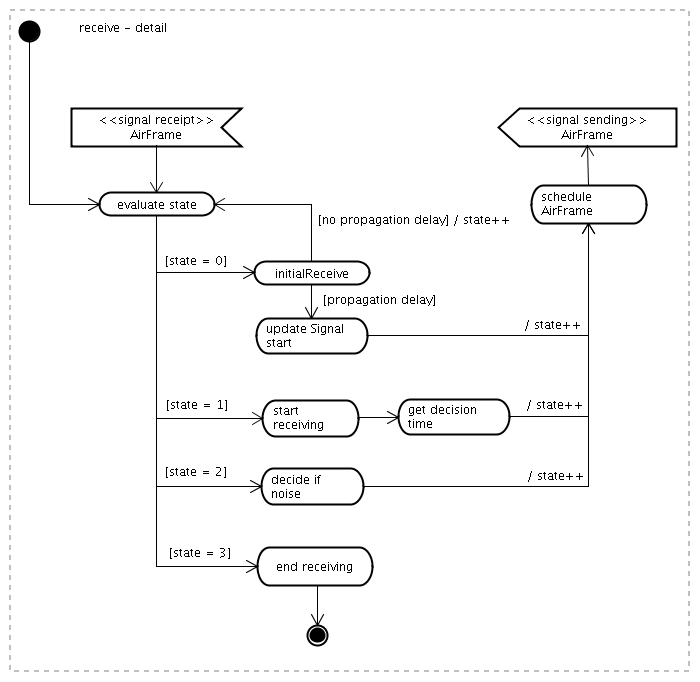
\includegraphics[width=340pt]{modelling/receive_detail.png}
 \caption{receive detail}
 \label{fig: receive detail}
\end{figure}

\begin{figure}[H]
 \centering
 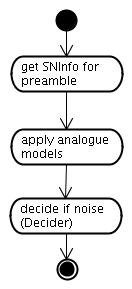
\includegraphics{modelling/end_preamble_detail.png}
 \caption{end preamble detail}
 \label{fig: end preamble detail}
\end{figure}

\newpage

%\subsection{provide status information to MAC}

%Passively provided information\req{provpassive}: \h{\baseMacLayer} is equipped with a reference to \h{\basePhyLayer} in order to obtain information
%about channelstate\req{channelstate} and current mode\req{currentmode} by
%simple method calls. \\
%Actively provided information\req{provactive}: A cMessage of the kind TX\_OVER
%is sent to MAC-Layer when a sending transmission is over\req{txover}, \saf{sending process}.

%\subsection{switch states}

%Furthermore the MAC-Layer is able to set the current mode (RX, TX, SLEEP)\req{switchmode} of the Phy-Layer by a simple method call.
%\h{\basePhyLayer} will change to switching state and schedule itself the appropriate timer for the switching interval\req{switchtimes}, \saf{mode state machine}.


%\subsection{send packets}

%Since \h{\baseMacLayer} has a reference to \h{\basePhyLayer} it can obtain information about the mode the radio is is currently in\req{sendPreqMode}, it is not already sending to the channel on its own\req{sendPreqSending} and the channel is idle\req{sendPreqIdle} via method calls, \saf{BasePhyLayer interface}.














